%\documentclass{article}


\documentclass[a4paper]{article}
\usepackage[utf8]{inputenc}
\usepackage[12pt]{extsizes}
\usepackage{amsmath,amsthm,amssymb}
\usepackage[hidelinks]{hyperref} 
\usepackage[warn]{mathtext}
\usepackage[T1,T2A]{fontenc}
\usepackage[utf8]{inputenc}
\usepackage[english,russian]{babel}
\usepackage{tocloft}
\linespread{1.5}
\usepackage{indentfirst}
\usepackage{setspace}
%\полуторный интервал
\onehalfspacing

\newcommand{\RomanNumeralCaps}[1]
    {\MakeUppercase{\romannumeral #1}}

\usepackage{amssymb}

\usepackage{graphicx, float}
\graphicspath{{pictures/}}
\DeclareGraphicsExtensions{.pdf,.png,.jpg}
\usepackage[left=25mm,right=1cm,
    top=2cm,bottom=20mm,bindingoffset=0cm]{geometry}
\renewcommand{\cftsecleader}{\cftdotfill{\cftdotsep}}

%\addto\captionsrussian{\renewcommand{\contentsname}{СОДЕРЖАНИЕ}}
%\addto\captionsrussian{\renewcommand{\listfigurename}{СПИСОК ИЛЛЮСТРАЦИЙ}}

\usepackage{fancyhdr}
\usepackage[nottoc]{tocbibind}

\fancypagestyle{plain}{
\fancyhf{}
\renewcommand{\headrulewidth}{0pt}
\fancyhead[R]{\thepage}
}

\usepackage{blindtext}
\pagestyle{myheadings}
\usepackage{hyperref}

\begin{document}
\begin{titlepage}
  \begin{center}
    \large
    Санкт-Петербургский политехнический университет Петра Великого
    
    Институт прикладной математики и механики
    
    \textbf{Высшая школа прикладной математики и вычислительной физики}
    \vfill
    \textsc{\textbf{\large{Отчёт по лабораторной работе №1}}}\\[5mm]
     по дисциплине\\ <<Математическая статистика>>\\
\end{center}

\vfill

\begin{tabular}{l p{140} l}
Выполнил студент \\группы 3630102/80401 && Веденичев Дмитрий Александрович \\
\\
Проверил\\Доцент, к.ф.-м.н.& \hspace{0pt} &   Баженов Александр Николаевич \\\\
\end{tabular}

\hfill \break
\hfill \break
\begin{center} Санкт-Петербург \\2021 \end{center}
\thispagestyle{empty}
\end{titlepage}
\newpage
\newpage
\begin{center}
    \setcounter{page}{2}
    \tableofcontents
\end{center}
\newpage
\begin{center}
    \setcounter{page}{3}
    \listoffigures
\end{center}

\newpage

\section {Постановка задачи}
\noindent Для 5 распределений:
\begin{enumerate}
	\item $N(x, 0, 1)$ -- нормальное распределение
	\item $C(x, 0, 1)$ -- распределение Коши
	\item $L(x, 0, \frac{1}{\sqrt{2}})$ -- распределение Лапласа 
	\item $P(k, 10)$ -- распределение Пуассона
	\item $U(x, -\sqrt{3}, \sqrt{3})$ -- расномерное распределение
\end{enumerate}

\noindent Сгенерировать выборки размером 10, 50 и 1000 элементов.
 
\noindent Построить на одном рисунке гистограмму и график плотности распределения.

\section {Теория}

\subsection{Распределения}
	\begin{itemize}
		\item Нормальное распределение \begin{equation}
										  N(x, 0, 1) = \frac{1}{\sqrt{2\pi}}e^{\frac{-x^2}{2}} \label{norm} 
									   \end{equation}
		\item Распределение Коши \begin{equation}
									C(x, 0, 1) = \frac{1}{\pi}\frac{1}{x^2+1} \label{koshi}
								 \end{equation} 
		\item Распределение Лапласа \begin{equation}
									   L(x, 0, \frac{1}{\sqrt{2}}) = \frac{1}{\sqrt{2}}e^{-\sqrt{2}|x|} \label{laplace} 
									\end{equation}
		\item Распределение Пуассона \begin{equation}
										P(k, 10) = \frac{10^k}{k!}e^{-10}\label{puasson}
									 \end{equation}
		\item Равномерное распределение \begin{equation}
				U(x, -\sqrt{3}, \sqrt{3}) =
				\begin{cases}
					\frac{1}{2\sqrt{3}} &\text{$при |x|\leq \sqrt{3}$}\\
					0 &\text{$при |x|>\sqrt{3}$}
				\end{cases}
				\label{uni} 
			\end{equation}
	\end{itemize}

	\subsection{Гистограмма}
	\subsubsection{Определение}
	 \textit{Гистограмма} в математической статистике — это функция, приближающая плотность вероятности некоторого распределения, построенная на основе выборки из него.
	
	\subsubsection{Графическое описание}
	 Графически гистограмма строится следующим образом. Сначала множество значений, которое может принимать элемент выборки, разбивается на несколько интервалов. Чаще всего эти интервалы берут одинаковыми, но это не является строгим требованием. Эти интервалы откладываются на горизонтальной оси, затем над каждым рисуется прямоугольник. 
	 
	 Если все интервалы были одинаковыми, то высота каждого прямоугольника пропорциональна числу элементов выборки, попадающих в соответствующий интервал. 
	 
	 Если интервалы разные, то высота прямоугольника выбирается таким образом, чтобы его площадь была пропорциональна числу элементов выборки, которые попали в этот интервал.
	
	\subsubsection{Использование}
	 Гистограммы применяются в основном для визуализации данных на начальном этапе статистической обработки. 
	 
	 Построение гистограмм используется для получения эмпирической оценки плотности распределения случайной величины. Для построения гистограммы наблюдаемый диапазон изменения случайной величины разбивается на несколько интервалов и подсчитывается доля от всех измерений, попавшая в каждый из интервалов. Величина каждой доли, отнесенная к величине интервала, принимается в качестве оценки значения плотности распределения на соответствующем интервале.

\section {Программная реализация} 	
Лабораторная работа выполнена на языке Python вресии 3.7 в среде разработки PyCharm. Использовались дополнительные библиотеки:\\ 
1. scipy\newline
2. numpy\newline
3. matplotlib\newline
4. math 

В приложении находится ссылка на GitHub репозиторий с исходныи кодом.

\section {Результаты} 

\subsection{Гистограммы и графики плотности распределения}
	\begin{figure}[H]
		\centering
		\begin{tabular}{ccc}
			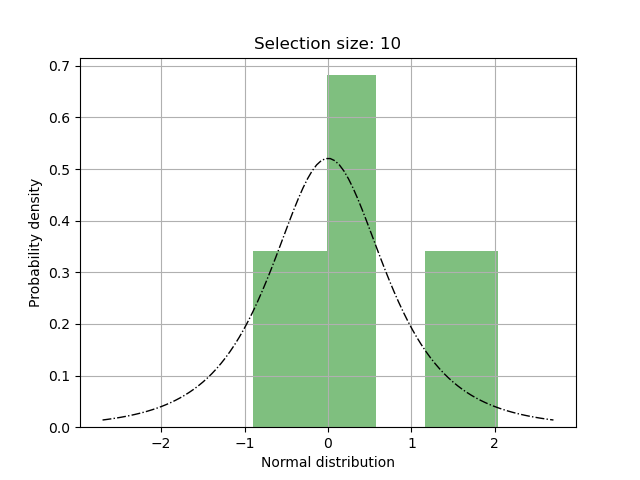
\includegraphics[width=55mm, height =0.25\textheight]{normal_10.png}
			&
			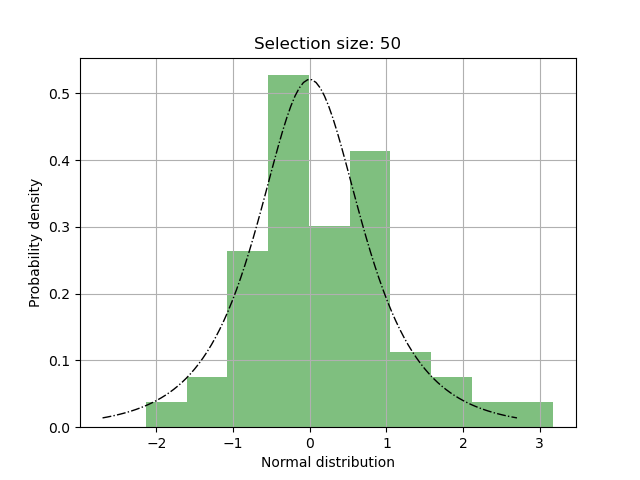
\includegraphics[width=55mm, height =0.25\textheight]{normal_50.png}
			&
			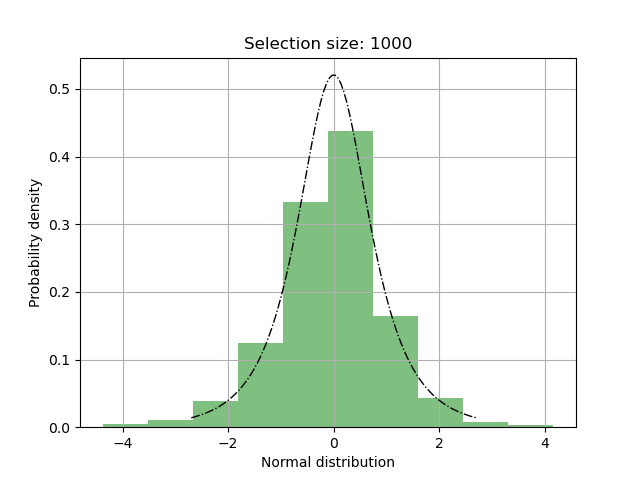
\includegraphics[width=55mm, height =0.25\textheight]{normal_1000.png}
		\end{tabular}
		\caption{Нормальное распределение \eqref{norm}} 
		\label{fig:normal}
	\end{figure}

	\begin{figure}[H]
		\centering
		\begin{tabular}{ccc}
			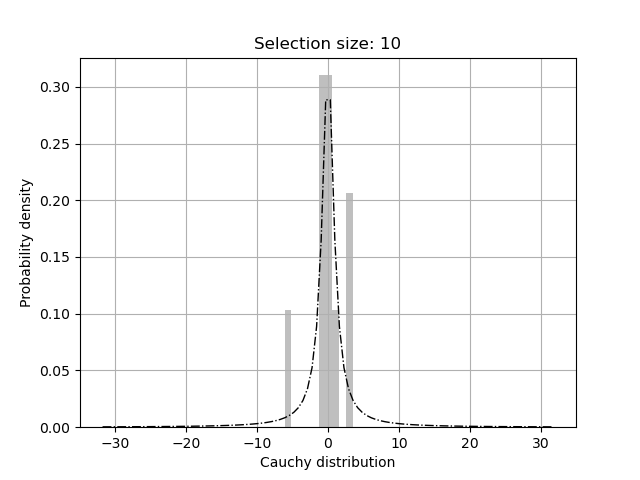
\includegraphics[width=55mm, height =0.25\textheight]{cauchy_10.png}
			&
			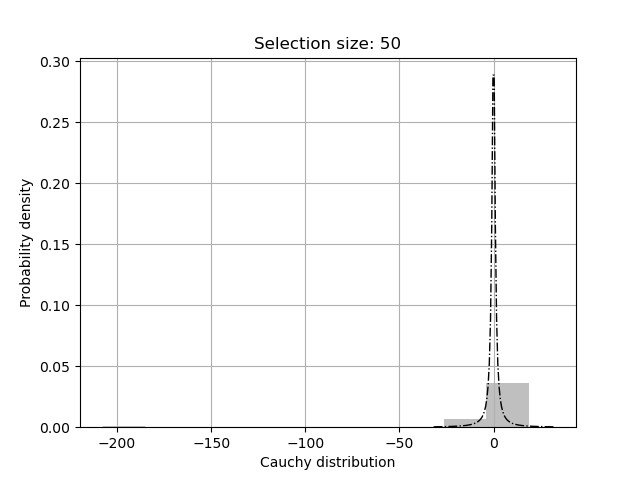
\includegraphics[width=55mm, height =0.25\textheight]{cauchy_50.png}
			&
			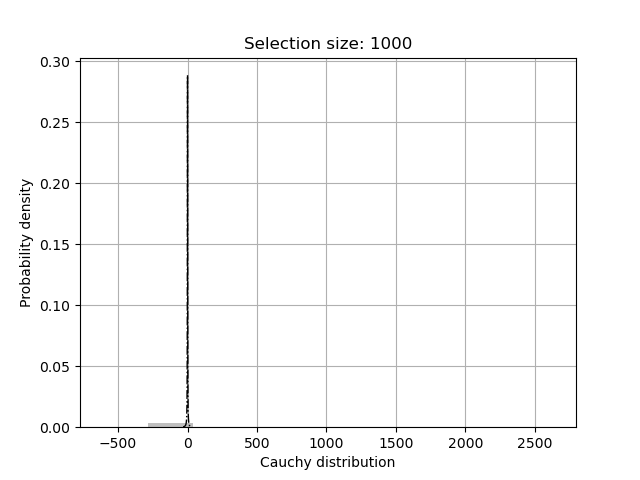
\includegraphics[width=55mm, height =0.25\textheight]{cauchy_1000.png}
		\end{tabular}
		\caption{Распределение Коши \eqref{koshi}}
		\label{fig:cauchy}
	\end{figure}
	

	\begin{figure}[H]
		\centering
		\begin{tabular}{ccc}
			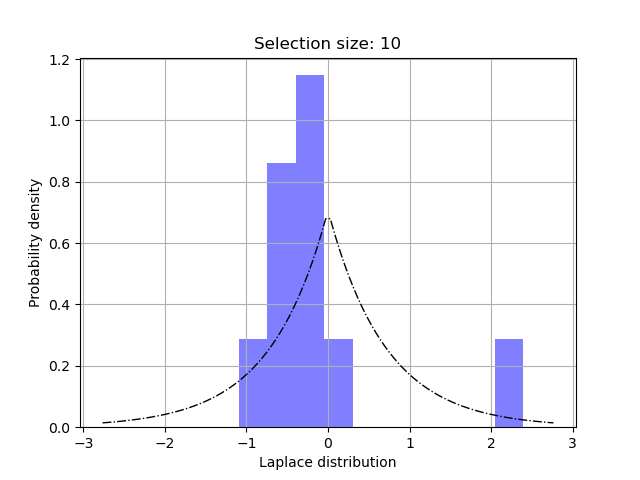
\includegraphics[width=55mm, height =0.25\textheight]{laplace_10.png}
			&
			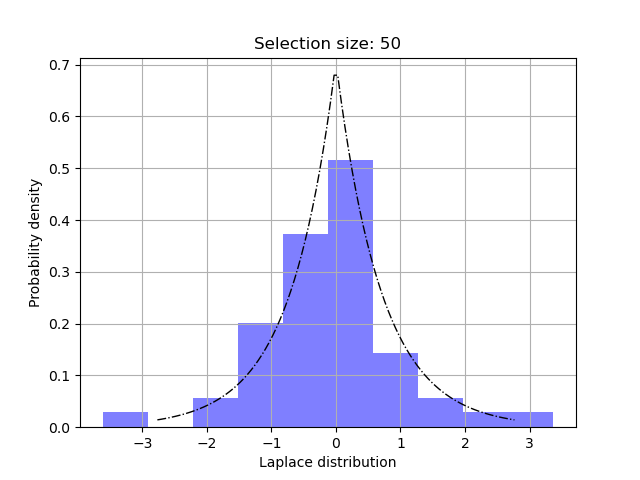
\includegraphics[width=55mm, height =0.25\textheight]{laplace_50.png}
			&
			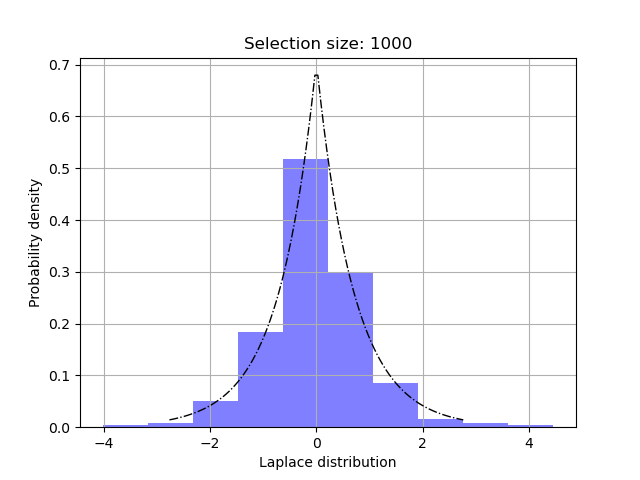
\includegraphics[width=55mm, height =0.25\textheight]{laplace_1000.png}
		\end{tabular}
		\caption{Распределение Лапласа \eqref{laplace}}
		\label{fig:laplace}
	\end{figure}


	\begin{figure}[H]
		\centering
		\begin{tabular}{ccc}
			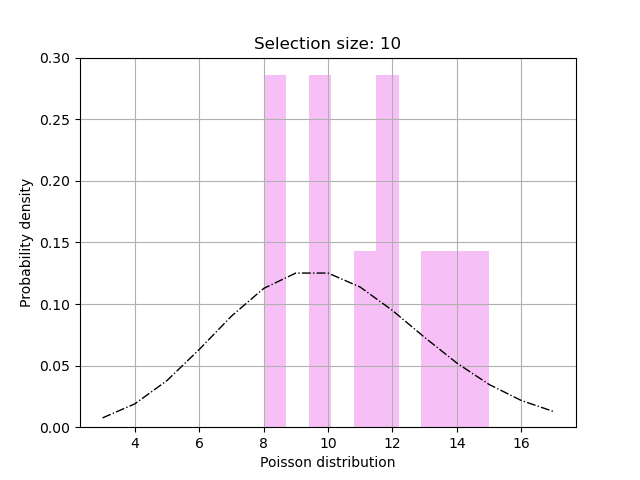
\includegraphics[width=55mm, height =0.25\textheight]{poisson_10.png}
			&
			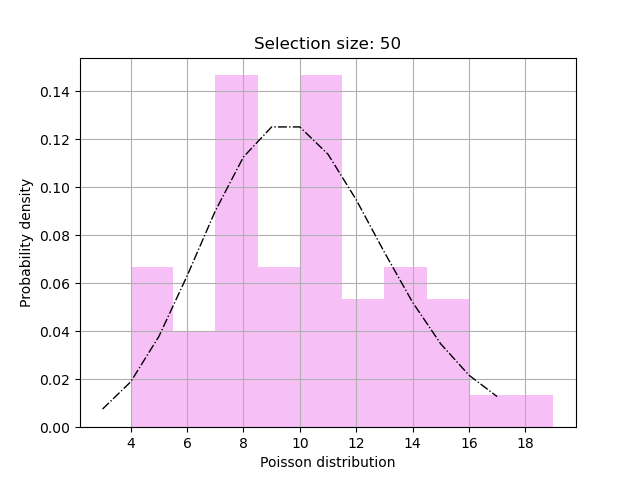
\includegraphics[width=55mm, height =0.25\textheight]{poisson_50.png}
			&
			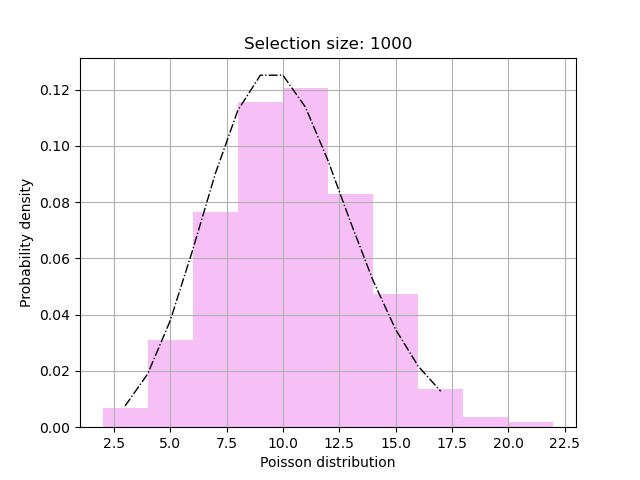
\includegraphics[width=55mm, height =0.25\textheight]{poisson_1000.png}
		\end{tabular}
		\caption{Распределение Пуассона \eqref{puasson}}
		\label{fig:poisson}
	\end{figure}


	\begin{figure}[H]
		\centering
		\begin{tabular}{ccc}
			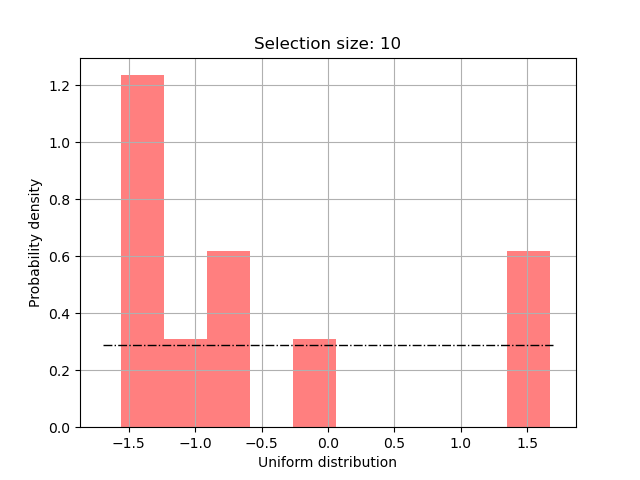
\includegraphics[width=55mm, height =0.25\textheight]{Uniform_10.png}
			&
			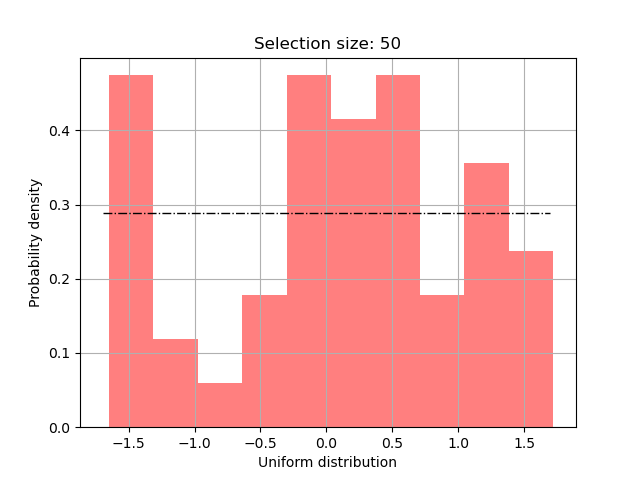
\includegraphics[width=55mm, height =0.25\textheight]{Uniform_50.png}
			&
			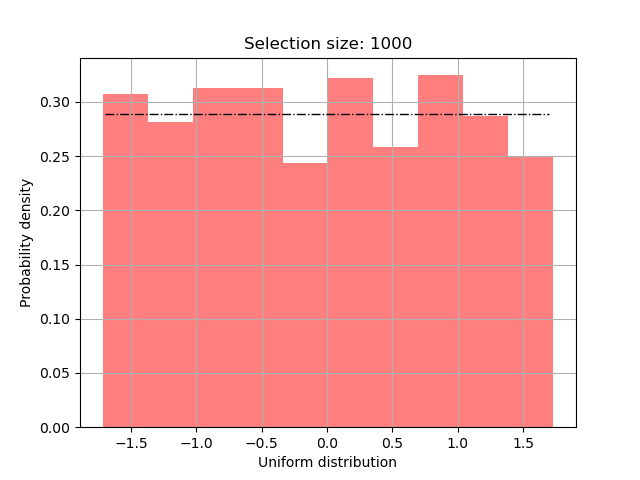
\includegraphics[width=55mm, height =0.25\textheight]{Uniform_1000.png}
		\end{tabular}
		\caption{Равномерное распределение \eqref{uni}}
		\label{fig:uniform}
	\end{figure}

\section{Обсуждение}

По результатам проделанной работы можем сделать вывод о том, что чем больше выборка для каждого из распределений, тем ближе ее гистограмма к графику плотности вероятности того закона, по которому распределены величины сгенерированной выборки. Чем меньше выборка, тем менее она показательна - тем хуже по ней определяется характер распределения величины.

Гистограммы составленные по маленькой выборке из 10 элементов не информативны.По ним нельзя определить по какому распределению они построены. С увеличением выборки до 50 элементов некоторые гистограммы(Лаплас, Нормальное, Пуассон) начинают принимать форму близкую к описываемым ими распределениям. На выборке из 1000 элементов можно однозначно определить равномерное распределение, распределение Пуассона. Гистограммы нормального распределения и распределения Лапласа вышли зеркальными.

 
Также можно заметить, что максимумы гистограмм и плотностей распределения почти нигде не совпали. Из полученных гистограмм, ближе всего к совпадению находятся гистограммы Лапласа(1000) и Пуассона(1000). Также наблюдаются всплески гистограмм, что наиболее хорошо прослеживается на распределении Коши. 

\section{Приложение}

\noindent Код программы GitHub URL:\\
\newline https://github.com/PopeyeTheSailorsCat/math\_stat\_2021/tree/main/lab1/src

\end{document}